
\documentclass[11pt]{report}
\usepackage {listings}
\usepackage {color}
\usepackage {graphicx}

\graphicspath{{./images/}}
\begin{document}

\title{DPA 8150 Project 1 Writeup}
\author{Galen M. Helfter\\
       }

% Code listing setup
\definecolor{dkgreen}{rgb}{0,0.6,0}
\definecolor{gray}{rgb}{0.5,0.5,0.5}
\definecolor{mauve}{rgb}{0.58,0,0.82}
\definecolor{dkred}{rgb}{0.58,0,0}

\lstset{frame=tb,
  language=Lisp,
  aboveskip=2mm,
  belowskip=2mm,
  showstringspaces=false,
  columns=flexible,
  basicstyle={\small\ttfamily},
  numbers=none,
  numberstyle=\tiny\color{gray},
  keywordstyle=\color{dkred},
  commentstyle=\color{dkgreen},
  stringstyle=\color{mauve},
  rulecolor=\color{black},
  breaklines=true,
  breakatwhitespace=true,
  tabsize=2
}

\centerline{\textbf{DPA 8150 Project 1}}
\centerline{\textbf{Galen M. Helfter}}

\bigskip
\textbf{Description:}

For this project, we were to implement an assortment of image operators, as
described in Brinkmann's {\it The Art and Science of Digital Compositing}.

For this project, I implemented the operations using the Common Lisp
language, along with a set of Tk bindings to use Tcl/Tk to drive the display.

The program only takes PNG images, and uses a binding and interface to some
C code that I've written to bring those images into the program. The code
is compiled to a shared object file, which can be linked to by Lisp and can
then be dealt with in the appropriate code for the application.

To run the code, SBCL needs to be installed. The makefile can then be called
normally to create the core file, which will then be run by the run.sh shell
script. The shell script will take up to three command line arguments as well,
to specify an image 1, an image 2 and a matte image. All of these currently
need to be of the same dimensions, I haven't yet implemented dimension
independent code.

\bigskip
\textbf{Simple operations}

To introduce the basic operations, the operation macro needs to first be
introduced. Each operation uses this macro to implement their functionality,
as it's easy to abstract the operation.

\begin{lstlisting}
(defmacro operation (img out ch i &body body)
  `(loop for ,i of-type fixnum from 0 to (- (image-dim ,img) 1) do
     (if (= (mod (channels ,img) 2) 0) ; Account for alpha channel
       (loop for ,ch from 0 to (- (channels ,img) 2) do
         (setf (aref (data ,out)
                    (+ (the fixnum (* ,i (channels ,out))) ,ch))
           (progn ,@body)))
       (loop for ,ch from 0 to (- (channels ,img) 1) do
         (setf (aref (data ,out)
                    (+ (the fixnum (* ,i (channels ,out))) ,ch))
          (progn ,@body))))))
\end{lstlisting}

\begin{figure}[h!]
\centering
    \includegraphics[width=8cm]{contrast}\includegraphics[width=8cm]{gamma}
\caption{Contrast and gamma operations}
\end{figure}

An example of the invert function is given here, using this macro.

\begin{lstlisting}
(defmethod invert ((img image) (out image))
  (operation img out ch (- 1.0 (access-pixels-sdim img i ch))))
\end{lstlisting}

Then, for required functionality, there are the contrast and gamma functions,
shown below. Monochrome is also shown, as it is needed later for lumakeying.

\begin{lstlisting}
(defmethod simple-contrast ((img image) (out image))
  (declare (optimize (speed 3) (safety 0)))
  (operation img out ch i (* (the single-float
                             (- (access-pixels-sdim img i ch)
                                0.33f0)) 3f0)))

(defmethod gamma-correct ((img image) (out image) gamma)
  (declare (optimize (speed 3) (safety 0))
           (type single-float gamma))
  (operation img out ch i (expt
                              (access-pixels-sdim img i ch)
                            (the single-float (/ 1f0 gamma))))

(defmethod monochrome ((img image) (out image))
  (declare (optimize (speed 3) (safety 0)))
  (operation img out ch i
    (+ (the single-float (* (access-pixels-sdim img i 0) 0.309f0))
       (the single-float (+ (the single-float
                              (* (access-pixels-sdim img i 1) 0.609f0))
                            (the single-float
                              (* (access-pixels-sdim img i 2)
                                 0.082f0)))))))
\end{lstlisting}

\begin{figure}[h!]
\centering
    \includegraphics[width=8cm]{edge}\includegraphics[width=8cm]{blur}
\caption{Edge detection and blur}
\end{figure}

\bigskip
\textbf{Convolve/spatial operations}

For this set of operations, I used mirroring to implement the convolution
on the edges, as can be seen in the given function, convolve-neighbor-dim.

\begin{lstlisting}
(defun convolve-neighbor-dim (d md dind)
  (cond
    ((>= (+ d dind) (- md 1))
     (- (- md 1) (- (+ d dind) (- md 1))))
    ((< (+ md dind) 0)
     (abs (+ d dind)))
    (t (+ d dind))))
\end{lstlisting}

The convolve operation uses a modified version of the operation macro, which
uses xy indices instead of just the i index. It works by destructively storing
the results of the filter multiplied by the appropriate pixel into an array,
then using a reduce call to aggregate them into the final result.

The median filter is more complicated, and some of the decisions have to do
with nuances in the way lisp does things, notably with the pairlis function.
The description of it is in the code, so I won't put it here as well.

\begin{figure}[h!]
\centering
    \includegraphics[width=8cm]{sharpen}\includegraphics[width=8cm]{median}
\caption{Sharpen and median filters}
\end{figure}

\begin{lstlisting}
(defmethod convolve-3 ((img image) (out image) filter)
  (declare (type (simple-array single-float (9)) filter))
  ;; Working array is declared outside the loop and altered destructively
  (let ((working (the (simple-array single-float)
                   (make-array 9
                     :element-type 'single-float
                     :initial-element 0f0))))
    (operation-xy img out ch op-x op-y
      (loop for y of-type fixnum from -1 to 1 do
          (loop for x of-type fixnum from -1 to 1 do
            (setf (aref working (+ (+ x 1) (* (+ y 1) 3)))
                  (* (aref filter (+ (+ x 1) (* (+ y 1) 3)))
                     (access-pixel img
                       (convolve-neighbor-dim op-x (width img) x)
                       (convolve-neighbor-dim op-y (height img) y)
                       ch)))))
      (reduce #'+ working))))
(defmethod median-3 ((img image) (out image))
  (let ((working (list nil nil)))
    (loop for y of-type fixnum from 0 to 2 do
      (loop for x of-type fixnum from 0 to 2 do
        (push 0.0 (car working)) (push 0 (cadr working))))
    (loop for op-y of-type fixnum from 0 to (- (height img) 1) do
      (loop for op-x of-type fixnum from 0 to (- (width img) 1) do
        ;; Instead of appplying a filter, this will construct a set of
        ;; lists, one with the brightness and the other with the index.
        (loop for y of-type fixnum from -1 to 1 do
            (loop for x of-type fixnum from -1 to 1 do
              (setf (elt (car working) (+ (+ x 1) (* (+ y 1) 3)))
                (get-value img
                  (convolve-neighbor-dim op-x (width img) x)
                  (convolve-neighbor-dim op-y (height img) y)))
              (setf (elt (cadr working) (+ (+ x 1) (* (+ y 1) 3)))
                 (+ (convolve-neighbor-dim op-x (width img) x)
                   (* (width img)
                      (convolve-neighbor-dim op-y (height img) y))))))
        ;; Now, out can have the element at index four (the middle) of the
        ;; sorted combination of the two lists, which can be paired with
        ;; the pairlis function. cdr is used over cadr, since pairlis stores
        ;; a pair of cons cells, not an actual list, so cdr gives us the
        ;; element, not the tail list like it does for a list.
        (let ((ind (cdr (elt (sort (pairlis (car working) (cadr working))
                                       #'< :key #'car) 4))))
          (loop for ch of-type fixnum from 0 to (- (channels img) 1) do
            (setf (aref (data out)
                    (+ ch (+ (* (channels out)
                      (+ op-x (* (width img) op-y))))))
                  (access-pixels-sdim img ind ch))))))))
\end{lstlisting}

\bigskip
\textbf{Compositing operations}

\begin{figure}[h!]
\centering
    \includegraphics[width=8cm]{mix}
\includegraphics[width=8cm]{gammaray}
\caption{Straight mix operation performed between the standard image and the
         image shown on the right}
\end{figure}

Like other operations coded before, much of the functionality can be leveraged
from the operation macro defined before. Here a matte can be applied using what
amounts to a simple mapping operation (fundamentally) to the image.

\begin{lstlisting}
(defun apply-matte (img out matte)
  (operation img out ch (* (access-pixels-sdim img i ch)
                           (access-pixels-sdim matte i ch))))
\end{lstlisting}

\begin{figure}[h!]
\centering
    \includegraphics[width=8cm]{keymix}
\includegraphics[width=8cm]{matte}
\caption{The result of a keymix operation given the split matte shown}
\end{figure}

The over operator is straightforward, as is the mix operator.

\begin{lstlisting}
(defun add-images (img-1 img-2 out)
  (operation img-1 out ch (+ (access-pixels-sdim img-1 i ch)
                             (access-pixels-sdim img-2 i ch))))

(defmethod mix-image ((img-1 image) (img-2 image) (out image) mv)
  (declare (optimize (speed 3) (safety 0))
           (type single-float mv)
           (type image img-1 img-2 out) (inline + *))
  (operation img-1 out ch i (+ (the single-float
                               (* (access-pixels-sdim img-1 i ch) mv))
                             (the single-float
                               (* (access-pixels-sdim img-2 i ch)
                                 (- 1f0 mv))))))


(defmethod over ((img-1 image) (img-2 image) (out image))
  (declare (optimize (speed 3) (safety 0)))
  (operation img-1 out ch i (+ (access-pixels-sdim img-1 i ch)
                               (* (- 1f0 (access-pixels-sdim img-1 i 3))
                                  (access-pixels-sdim img-2 i ch)))))
\end{lstlisting}

\begin{figure}[h!]
\centering
    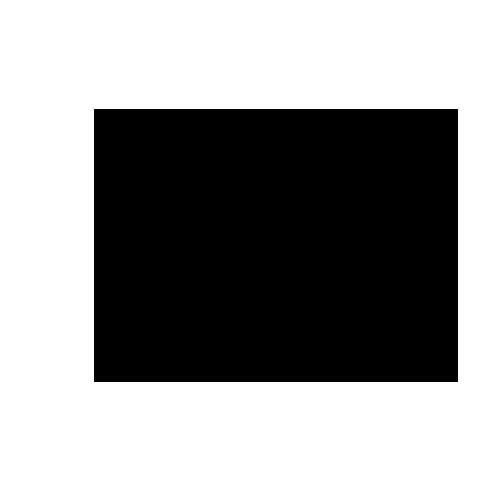
\includegraphics[width=8cm]{test_over}\includegraphics[width=8cm]{over}
\caption{Testing the over operator with this black rectangle}
\end{figure}

The key mix operation is simple as well, being a combination of the previous
matte applying code along with the addition operatior.

\begin{lstlisting}
(defun keymix (img-1 img-2 out matte)
  (declare (type image img-1 img-2 out))
  (let* ((temp-1 (make-instance 'image :width (width img-1)
                                       :height (height img-1)
                                       :channels (channels img-1)))
         (temp-2 (make-instance 'image :width (width img-1)
                                       :height (height img-1)
                                       :channels (channels img-1))))
         (invert matte temp-1) ; Perform operation with inverse first
         (apply-matte img-2 temp-2 temp-1)
         (apply-matte img-1 temp-1 matte)
         (add-images temp-1 temp-2 out)))
\end{lstlisting}

\bigskip
\textbf{Keying and matte creation}

Keying was a little more difficult for especially the chroma key. The luma key
is simple, as shown below, along with the color difference method for blue.

\begin{figure}[h!]
\centering
    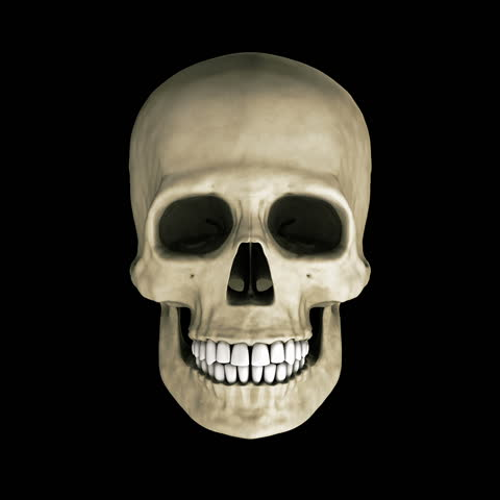
\includegraphics[width=8cm]{skull}\includegraphics[width=8cm]{lumakey}
\caption{Luma keying performed on this skull}
\end{figure}

\begin{lstlisting}
(defmethod luma-key ((img image) (out image))
  (monochrome img out)
  (simple-contrast out out))
(defmethod color-difference-blue ((img image) (out image))
  (loop for i of-type fixnum from 0 to (- (image-dim img) 1) do
   (let* ((r (access-pixels-sdim img i 0))
          (g (access-pixels-sdim img i 1))
          (b (access-pixels-sdim img i 2)))
     (if (> b g) (setf b g))
     (loop for ch of-type fixnum from 0 to (- (channels img) 1) do
       (setf (aref (data out) (+ ch (* i (channels img))))
             (aref (data img) (+ ch (* i (channels img))))))
     (setf (aref (data out) (+ 2 (* i (channels img)))) b))))
(defmethod color-difference-blue-matte ((img image) (out image))
  (loop for i of-type fixnum from 0 to (- (image-dim img) 1) do
    (let* ((r (access-pixels-sdim img i 0))
           (g (access-pixels-sdim img i 1))
           (b (access-pixels-sdim img i 2)))
      (setf b (- b (max r g)))
      (setf (aref (data out) (+ 0 (* i (channels img)))) b)
      (setf (aref (data out) (+ 1 (* i (channels img)))) b)
      (setf (aref (data out) (+ 2 (* i (channels img)))) b))))
(defmethod chroma-key ((img image) (out image) hue)
  (declare (type single-float hue))
  (loop for i of-type fixnum from 0 to (- (image-dim img) 1) do
     (let* ((r (access-pixels-sdim img i 0))
            (g (access-pixels-sdim img i 1))
            (b (access-pixels-sdim img i 2)))
       (cond ((< (abs (- (rgb-to-hue r g b) hue)) *hue-eps*)
              (setf (aref (data out) (+ 0 (* i (channels img)))) 0.0)
              (setf (aref (data out) (+ 1 (* i (channels img)))) 0.0)
              (setf (aref (data out) (+ 2 (* i (channels img)))) 0.0))
             (t (loop for ch of-type fixnum from 0 to (- (channels img) 1) do
                  (setf (aref (data out) (+ ch (* i (channels img))))
                        (aref (data img) (+ ch (* i (channels img)))))))))))
\end{lstlisting}

\begin{figure}[h!]
\centering
    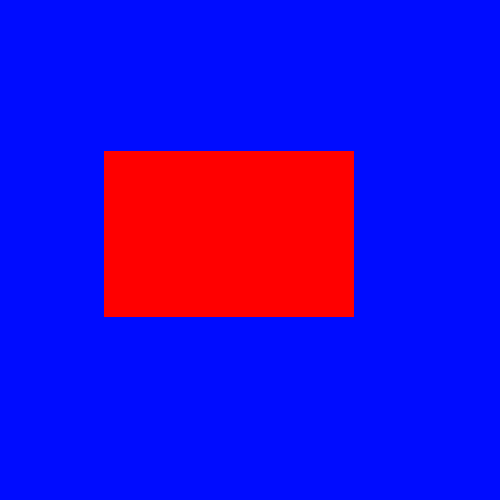
\includegraphics[width=4cm]{test_chroma}\includegraphics[width=4cm]{chroma}
    \includegraphics[width=4cm]{diff}
\caption{Chroma key, before and after, and then the color difference on blue}
\end{figure}

\bigskip
\textbf{UI Code}

For the UI code, the most noteworthy pieces are some of the functions in the
{\it interface.lisp} file. With tk, it is surprisingly difficult to get it
to display an image dynamically, which is needed for compositing operations.
After a long time, while contemplating writing the image to disc and allowing
tk to read it, I managed to get something proper working. The
ltk:image-writedata function used is one that I wrote and added to the
{\it ltk.lisp} file, which calls wish with the {\it image put data} command in
Tcl/tk. Then, I had to find a way to get some data it would take. Finally, I
wrote a function to generation a hex string of the image, with a \# starting
each pixel and each row contained in a set of brackets, as the Tcl library is
expecting the pixels to be in a Tcl list. These important functions are as
follows:

\begin{lstlisting}
(defun image-writedata (image data)
  (format-wish "~A put \"~a\"" (name image) data))
(defun image-to-hex-string (img)
  (declare (optimize (speed 3) (safety 0)) (type image img))
  (let* ((rval (make-array (+ (* 2 (image-size img))
                              (image-dim img) (image-dim img)
                              (* 4 (height img)))
                           :element-type 'character
                           :fill-pointer 0)))
    (loop for y of-type fixnum from 0 to (- (height img) 1) do
      (vector-push #\{ rval)
      (vector-push #\Space rval) 
      (loop for x of-type fixnum from 0 to (- (width img) 1) do
        (let* ((r (to-8bit (access-pixel img x y 0)))
               (g (to-8bit (access-pixel img x y 1)))
               (b (to-8bit (access-pixel img x y 2)))
               (r-str (write-to-string r :base 16))
               (g-str (write-to-string g :base 16))
               (b-str (write-to-string b :base 16)))
          (declare (type simple-string r-str g-str b-str))
          (vector-push #\# rval)
          (cond ((< r 127)
                 (vector-push #\0 rval)
                 (vector-push (char r-str 0) rval))
                (t
                 (vector-push (char r-str 0) rval)
                 (vector-push (char r-str 1) rval)))
          (cond ((< g 127)
                 (vector-push #\0 rval)
                 (vector-push (char g-str 0) rval))
                (t
                 (vector-push (char g-str 0) rval)
                 (vector-push (char g-str 1) rval)))
          (cond ((< b 127)
                 (vector-push #\0 rval)
                 (vector-push (char b-str 0) rval))
                (t
                 (vector-push (char b-str 0) rval)
                 (vector-push (char b-str 1) rval))))
        (vector-push #\Space rval))
      (vector-push #\} rval)
      (vector-push #\Space rval))
    rval))

\end{lstlisting}

\end{document}
